\section{Wireless Basics}

\begin{figure}[h]
	\centering
	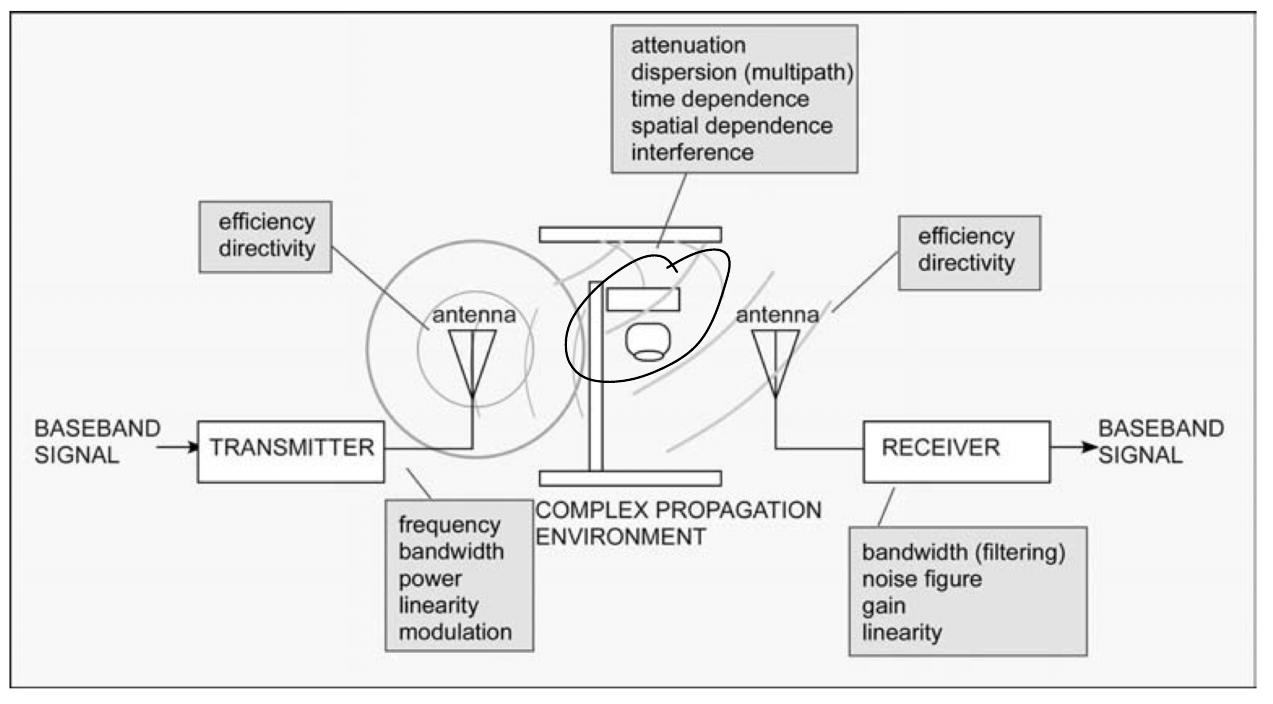
\includegraphics[scale=0.4]{images/1-wireless-system.png}
	\caption{A wireless system, its basic components and characteristic measures}
	\label{fig:wireless-system}
\end{figure}

\paragraph{Radio Frequency Signal}
Electromagnetic radiation, with waves being created in the antenna by an alternating current at the desired frequency.
Mathematically described as a function of the time $t$:
$$ v(t) = A \sin (2 \pi f t + \phi) $$
with amplitude $A$, frequency $f$ and phase $\phi$.
Also recall that the period is $T = \frac{1}{f}$ and the wavelength (distance travelled during one period) is $\lambda = \frac{v}{f}$ (usually $v=c$ speed of light).

\paragraph{Bandwidth}
The capacity of a communications link to transmit the maximum amount of data from one point to another over a connection in a given amount of time (in bits per second bps). 
An analogy: The amount of water that can flow through a water pipe.

In other words, the measure of frequency content of the signal.
E.g. the human voice contains frequencies in the range from 30 Hz to 10 kHz, and the bandwidth of a single 802.11 channel is 22 MHz.

Note that often the bandwidth of the baseband and that of the carrier (and thus that of the modulated signal) differ!
E.g. see spread spectrum techniques.
% TODO link to section

\begin{figure}
	\centering
	
\includegraphics[scale=0.35]{images/1-wifi-channels.png}
	\caption{2.4 GHz WiFi Channels \href{https://en.wikipedia.org/wiki/List\_of\_WLAN\_channels\#/media/File:2.4\_GHz\_Wi-Fi\_channels\_(802.11b,g_WLAN).svg}{[Source]}}
	\label{fig:wifi-channels}
\end{figure}

\paragraph{Baseband}
An original transmission signal that has not been modulated or has been demodulated to its original frequency.
I.e. the actual \textbf{information signal}.
Most telecommunication protocols require baseband signals to be converted, or modulated, to a higher frequency in order to be transmitted over long distances.

\paragraph{Carrier}
A transmitted electromagnetic pulse or wave at a steady base frequency of alternation on which information can be imposed.
Typically a pure sinusoid of a particular frequency and phase that carries the information.
Usually the frequency of the carrier is much higher than that of the baseband.

\paragraph{Modulated Signal}
A carrier that has been loaded or modulated with the information signal.

\paragraph{Modulation}
Process of imposing the baseband onto the carrier.
The baseband is used to alter one aspect of the carrier, such as:
signal strength (\textit{amplitude modulation AM}), frequency (\textit{frequency modulation FM}), phase (\textit{phase modulation PM}).
In other words, one of the values $A, f, \phi$ in the above equation of the signal is manipulated.

\paragraph{Phase-shift keying PSK}
Modulation technique varying the phase of the carrier.
Used e.g. in WiFi, RFID, Bluetooth.
Specific versions include Binary PSK, Quadrature PSK and Differential PSK.
Simple example: if the baseband bit is 0 do nothing to the carrier, if it is 1 shift the carrier phase by $\pi$.

\paragraph{I-Q Signal Representation}
A pair of periodic signals are said to be in ‘quadrature’ when they differ in phase by 90 degrees (e.g. the sine and cosine wave).
The ‘in-phase’ or reference signal is referred to as ‘I’ (conventionally cosine), and the signal that is shifted by 90 degrees (in quadrature) is called ‘Q’ (conventionally sine).
Used to represent modulations.

\paragraph{Antenna}
Interface between radio waves in the air and electric alternating currents in a conductor.
Types include: omni/dipole, yagi, horn, cantenna.

The directionality of an antenna described how well it transmits/receives into a particular direction.
\begin{itemize}
	\item \textbf{isotropic} -- Theoretical, radiates with the same intensity equally in all directions. Often used as a reference antenna when calculating the gain.
	\item \textbf{omni-directional} -- Radiates equally well in all directions in a flat horizontal plane. Most common types in consumer devices.
	\item \textbf{directional} -- Radiates best in a given direction by focussing its power. Can thus work with weaker signals than an omni-directional antenna of the same power.
\end{itemize}

\begin{figure}
	\centering
	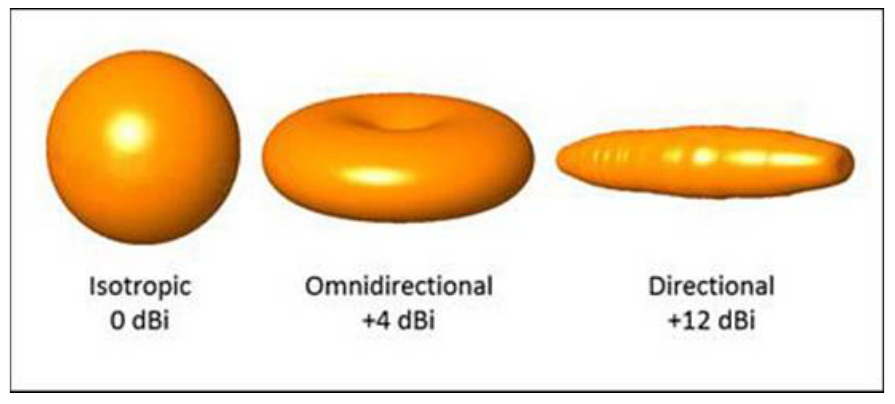
\includegraphics[scale=0.4]{images/1-directionality.png}
	\caption{Antenna directionality}
	\label{fig:directionality}
\end{figure}

\paragraph{Phased Array}
Array of fixed antennas where the phase of each signal is dynamically adjusted so that the signal will be in phase for a given direction.
Allows \textit{beam steering} towards a specific direction.
Possible applications? Can it be used to achieve security (e.g. confidentiality)?

\begin{figure}
	\centering
	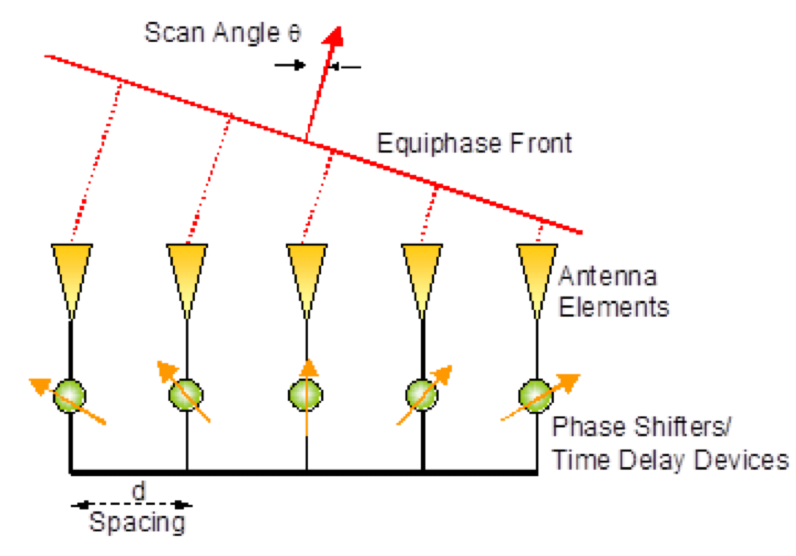
\includegraphics[scale=0.4]{images/1-beam-steering.png}
	\caption{Beam steering}
	\label{fig:beam-steering}
\end{figure}

\paragraph{Transmitter/Receiver}
Converts from digital to analogue, applies modulation and connects to the antenna (and vice versa).
Properties: transmitted power, carrier frequency, information bandwidth, modulation type, receiver sensitivity.

\paragraph{Software Defined Radio SDR}
Flexible, low-cost transmitter/receiver.
Implements components (mixer, amplifier, de-/modulator) in software rather than processing the signal in hardware.

\paragraph{Channel equation}
See \autoref{fig:signal-strength}.

signal strength at the receiver = transm. power + transm. antenna gain $-$ link loss + receiv. antenna gain

Note that in free space the power density of an EM wave obeys the inverse-square law:
$$ p \propto \frac{1}{d^2} $$

\begin{figure}
	\centering
	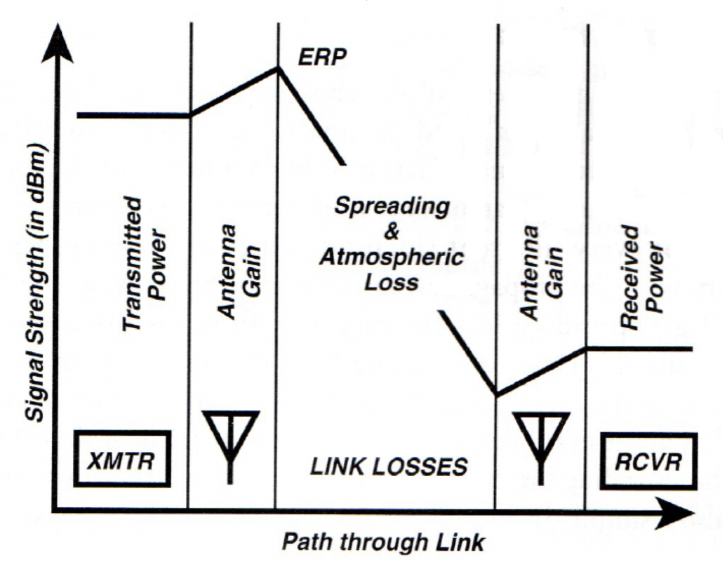
\includegraphics[scale=0.4]{images/1-signal-strength.png}
	\caption{Signal strength across the channel (ERP = Effective Radiated Power)}
	\label{fig:signal-strength}
\end{figure}

\paragraph{Receiver sensitivity}
The weakest signal from which the receiver can still obtain the desired information signal.
Depends not just on the antenna gain, but also on other factors such as the noise.

\paragraph{Decibel}
\begin{itemize}
	\item dBm -- signal strength in dB / 1 milliwatt mW
	\item dBW -- signal strength in dB / 1 watt W
	\item dBi -- antenna gain in dB / antenna gain of isotopic antenna in dB
\end{itemize}
Calculating a value in dB:
$$ dB(n) = 10 \log_{10} (n) \quad \text{ and } \quad dBm(n) = 10 \log_{10} (n / 1 mW) $$

\paragraph{Power Spectral Density diagram}
Depicts the power density (in dB) for a range of frequencies.
In simple terms, it shows how strong the signal is at a given frequency.


\paragraph{Security Goals}
Reasons: \textit{security} (integrity, confidentiality, authentication), \textit{regulatory} (personal liability for misuse of one's network access), \textit{safety} (RF-enabled implants).

Just reducing transmission power, hoping that the attacker will be too far away to listen on / send / modify messages, is NOT a solution.
In fact, WiFi signals can be received 10 km away, and similarly Bluetooth at 1 km distance (with good, directed equipment).

Example: \textit{passive keyless entry and start systems (PKES)}, i.e. wireless car keys.
Wrongly assume communication implies physical proximity (relay attack).
Needs: Authenticated proximity verification, message authentication.
